%!TEX root = ../Thesis.tex
\chapter{Introduction to tools of supervised machine learning}
\label{chap_introStat}

\section{Supervised machine learning to predict and to learn}
Supervised machine learning covers regression, classification and probability estimation models built on labeled data. Regression is to predict scalars (numbers), classification to predict class membership or lastly to rather predict a probability distribution across classes. 

The direct motive of supervised modeling is to predict a certain target information, that is otherwise expensive/tedious to measure, or only reveal it self in the future, or the measuring is invasive and will destroy the object of interest. The target is predicted by learning a simple or perhaps complex relationship between easy accessible features and the target from a labeled training data set. When a useful relationship has been established with a model, target predictions can be made for a unlabeled data set without the target.

An indirect motive of supervised machine learning is to elucidate a general relationship between features and targets. One example of an indirect motive is when modeling the contraceptive method choice reference data set \cite{lichman2013uci}, see also results part of forest floor article in Section \ref{article:forest}. Here, +1000 Indonesian married women had answered a questioneer on contraception and socio-economic status. To build a model to accurately predict contraception method choice based on 10 questions on socio-economic status was never the actual motive. It has little practical use to ask 10 questions to only estimate one answer. Why not just ask the right question at first? However, the structure of an accurately predicting model can be an useful empiric proposal for a general relationship. Scientifically, the next step is to form testable causal link theories inspired by the captured empiric relationships. 

\begin{figure}[!htbp]
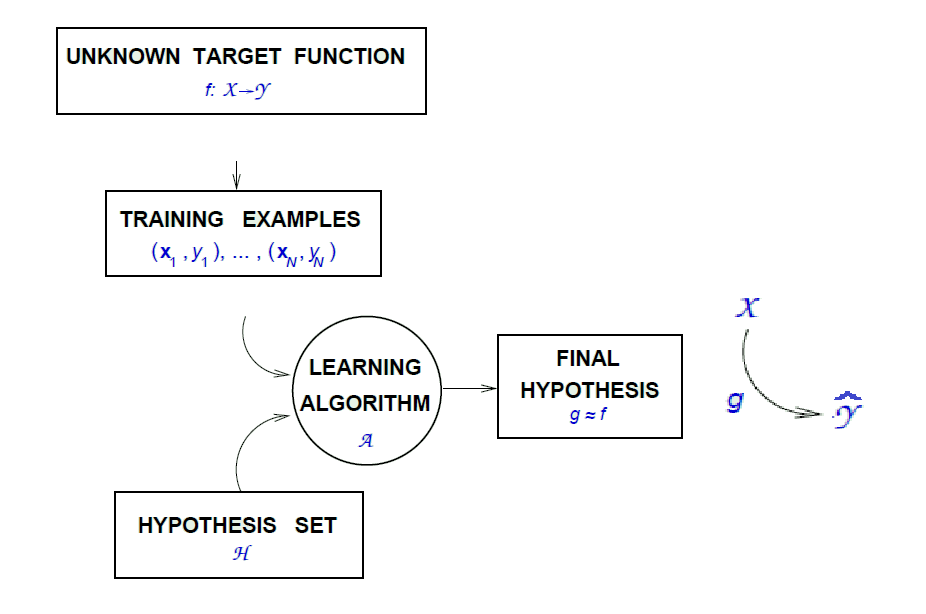
\includegraphics[width=\textwidth,height=\textheight,keepaspectratio]{graphics/sketchMLmapping.png}
\caption{We can imagine an unknown target function $f$ in nature, that generates the $N$ observed training examples $X_i$ $y_i$ for $i \in 1,2,...,N$. With a hypothesis set $H$, that is the set of hyper parameters we will try for $A$. Each hypothesis will yield a model. With model selection one final hypothesis and the resulting model $g$ is chosen. The model $g$ is a function that mimics $f$. With $g$ we can start to predict how $f$ behaves (direct motive), or secondary evaluate the structure of $g$ to both challenge the validity of $g$ and our current beliefs of $f$.
The figure is copied from a set of Caltech lecture slides \cite{Mostafa2013learning}.
}
\label{modelPredictExplain}
\end{figure}

A typical labeled data set, is organized as a data table with one column with desirable target information and a series of columns with feature information. Every row is an independent observation of one target and some features. A practical example is the public abalone data set. Here, a marine biologist may be interested in estimating the age of abalones (shellfish). However, determining age is tedious and requires to sacrifice each specimen to study the broken shell under a microscope after chemical staining. To measure the size and weight and to observe the gender is in contrary easy \cite{lichman2013uci}. Therefore the marine biologist can use a supervised regression model to learn a relationship between morphology and age, and use this relationship to predict effortless the age of new specimens. Each row of the data set will be one abalone randomly sampled from the ocean, a target column ($y$) will describe the age of each abalonem, and feature columns will describe other features measured.

\subsection{Univariate regression}
Perhaps a single feature such as weight ($x_{.1}$) would be almost perfectly linear related to age ($y_.$). In such case uni-variate linear regression (ordinary least squares) would be a sufficient model. Where $\hat{y} = b_1 x_{.1} + b_0$, and where $b_1$ and $b_0$ are chosen to minimize a loss function evaluating the training error. Let $x_{.1}$ be a vector of weight measurements and let $y_.$ be a vector age. Both $x_.1$ and $y_.$ are of length $N$, the sample size of the training set, and the elements are enumerated from $1$ to $N^{th}$ observation by $i$, such that $y_i$ is the age of the $i^{th}$ abalone, and $x_{i1}$ is the weight.

Perhaps the absolute abalone growth rate increases with age, and therefore the age of larger abalones are in general overestimated. By plotting the relationship and inspecting the residuals it may be evident, that linear fit is not optimal. To overcome this, the model may manually be expanded with a quadratic term such that $\hat{y} = b_2 x_{.1}^2 + b_1 x_{.1} + b_0$.  Thus in this manual approach, first a linear fit was made, and by inspecting the residuals it was obvious that transforming the weight measurements by non-linear quadratic transfer function would improve the linear relationship.

\subsection{Multiple linear regression and interaction terms}
The user may now start to include several transposed features and interaction terms. There is no direct limitation in linear regression to not model non-linear relationships and interactions terms. All these terms just have to be stated manually. For a small set of features, and where the goodness-of-fit of a linear model is already fair, it is easy to inspect the residuals to observe, how a linear fit may be inadequate. Hereafter one can specify some useful transfer functions and interaction terms to obtain an even better model. However, when the number of features become large, it will become tedious to manually state terms in the model. If the feature relationship is fairly complex (many interaction terms and non-linearities), then no two-dimensional residual plot can reveal what transfer functions to use. A fast fix is to state a model with several transfer functions for each feature and interactions for each pair of features.

One limitation is the degrees of freedom. In a linear ordinary least squares model, if the number of parameters to fit in the model outnumbers the number of observations, there is no longer one unique fit with a minimal loss function score, but rather a subset of solutions all with a constant error. It takes only an offset and a slope to connect two points with a line, or an offset and two slope coefficients to describe a plane connecting three points. Likewise, 18 points can always be connected by an 17-dimensional hyper plane plus an offset. The accuracy of a model should not be evalauted by training error, especially when then number of parameters are close to as many observations and/or if the observations are noisy.

\begin{quotation}
"With four parameters I can fit an elephant, and with five I can make him wiggle his trunk"  - J Neumann
\cite{wiki2016John}
\end{quotation}

Psychologist and economist Daniel Kahneman noted when working with notoriously noisy data from psychology tests, that multiple linear regression models explained the training data well, however the established model predicted poorly future results and could not be reproduced. Each subject (person) would be exposed to a number of sub tests outputting score values. Each sub test was designed to be related to e.g. leadership performance by some measurable definition. The test scores could be combined to predict future leadership for interviewed candidates with a multiple linear regression model, however Kahneman preferred to simply use the summed total score as a predictor, thus giving each sub test the same weight. He found this approach more accurate and reproducible than multiple linear regression \cite{kahneman2011thinking}.

The individual psychological tests aimed to reflect the same target and these were likely linearly related (collinearity). Moreover, the psychological observations were inherently noisy and the training set size modest. This was a recipe for a poor overfitted multiple linear regression model. The best ordinary least sqaures fit may be a spurious ratio between the sub tests, where some tests even are accredited by a negative coefficient, although having a positive linear relationship to the target.

Kahnemans practice of forcing all tests to have the same coefficient size is in practice the same as regularization, although a fairly crude version. A more elegant regularization method is the elastic net (EN). EN regression allow to do anything between classic multiple regression and a very strong regularization where all coefficient tend to have low values of equal size. Regularization tend to even the dependency on all features, unlike using only one feature greedily. Intuitively, to rely more evenly on different information sources under noisy conditions will lead to more robust models. Secondly increased regularization tend to prevent finding some very specific ratio between correlated features to explain the target, but rather use the weighted average of correlated features to predict.

The elastic net coefficient estimation Elastic-net do not only minimize squared target residuals but also the squared coefficents (L2/lambda penalization) and absolute coeeficients (L1/alpha penalization). An elastic net algorithm will likely use a convex optimization search to find the coefficients that minimizes this loss function,

\begin{equation}
\hat{\beta}_{elastic_{net}}  = 	\underset{\beta}{\argmin} 
\sum_{i=1}^{N} (y_i - \hat{y})^2 + 
\sum_{j=1}^{p} \lambda(
	 \alpha       \beta_j^2 + 
    (\alpha -1) | \beta_j |
) \quad ,
\end{equation}

where $N$ is the number of observations/rows, and $\hat{y}_i$ is the $i^{th}$ prediction $\hat{y}_i = \beta_0 + \beta_{1:p} x_i.$ and $p$ is the number of features/columns \cite{friedman2001elements}. The $\lambda$ and $\alpha$ parameter are specified before the convex optimization search. $\lambda$ controls the overall penalization of coefficient sizes. $\alpha$ is a value between 0 and 1. When $1$, only the sum squared coefficents is penalized ($L2$), whereas for $alpha=0$ only the sum of absolute coefficients is penalized ($L1$). Any value in between is a linear combination. Strict $L2$ penalization can never drive a coefficient entirely down to zero, as squaring a small number below $1$ makes it even smaller. With the $L1$ penalization it is possible to drive coefficients down to zero, thus effectively omitting them from the model. $L1$ penalization can be used for feature selection \cite{friedman2001elements}.

The elestic net estimator allow to introduce two types of gradual regularization driving down the effective number of parameters in the model. Elastic net can be seen as a learning algorithm $A$ that takes a training set $T$ ($(x_1,y_1),...,(x_N,y_N)$) and a set of hyper parameters $H$ ($\alpha$ and $\lambda$) as input. The leaning algorithm will then output a model function $g = A(T,w)$. The model function can make predictions $g(x_i)=\hat{y}_i$. The hyper parameters $\alpha$ and $\lambda$ should be chosen to obtain the lowest future prediction error and not necessarily to obtain the lowest training error, as the ordinary least squares fit do. To estimate what model will work best with future predictions cross-validation is used.

\section{Cross-validation}
There are infinite models that can explain a given training set perfectly. Especially a sufficient complex model, can always connect the dots in some way. In hind sight virtually anything can be explained. Cross-validation is a simulation of how well a given model will predict unseen data.

There are alternatives to cross-validation such as the 'Akaike information criterion' which will weight training set prediction accuracy against a penalty for model complexity. However the Akaike information criterion do not translate well to non-linear algorithmic models where the effective degrees of freedom is difficult to estimate.

Cross-validation is performed for two purposes. First, model selection, that is to compare our set of hypotheses to choose the most promising approach. In practice that is to select the most useful learning algorithm and optimize the hyper parameters and perhaps perform some feature selection. Secondly, to estimate the prediction error for future data generated by the same underlying function $f$ for a given built model $g$ \cite{friedman2001elements}.

\subsection{Segregation}
The simplest cross-validation scheme is segregation. The data set of data examples is randomly divided into e.g. 50\% training observations, 25\% validation (aka. calibration) and 25\% test observations. The learning algorithm uses the training set to estimate model parameters, the validation set is used to choose the hyper parameters of learning algorithm and the test set is used to estimate the future prediction error \cite{friedman2001elements}.

\subsection{Unbiased estimation of prediction error}
\label{unbiased_estimation}
To perform model selection and to estimate prediction error is often the same procedure. However, especially if the set of model hypotheses is large, there may be some hypotheses, that only by chance produced a good model fit of the validation set. Selecting the hypothesis with lowest validation error may be the best strategy, however the low validation error of this hypothesis is an inseparable combination of skill plus luck. Where the skill component remains, the luck component is inherently non reproducible and will regress towards the mean \cite{kahneman2011thinking}. Thus, we don't know exactly why a given hypothesis turned out to be the best to fit the validation set. The best hypothesis will subsequently most likely perform worse on the test set than on the validation set, as luck is difficult to reproduce. For a large hypothesis set, where all models have a low explained variance, we should expect the luck component to be substantial. The \textit{Inverse gamblers fallacy} would be the extreme cases, where there is no skill and only luck. A gambler may erronously believe that she should keep playing, as she has been in luck the last couple of rounds. An extended version of the \textit{Infinite monkeys theorem} explains the problem well. Theoreme states, that in a room sit infinite monkeys and type randomly on type writers, one monkey will eventually  have written the complete works of Shakespeare. Would you hire this monkey expecting it to write more brilliant works in the future? \cite{wiki:gamblers,monkeys}

This problem is very related to family-wise error of multiple hypotheses testing in classical statistics and e.g. the Tukey and Bonferoni corrections. However no such corrections exists for general machine learning.

In conclusion when ever making a model selection or a parameter estimation based on a set of data, the same data set cannot provide an unbiased estimation of the model performance. A new cross-validation must be wrapped around the current procedure. Lastly also within machine learning literature, publication bias inevitably exists. An article including a model procedure with a good final test score, is more likely to be submitted and accepted. But as a component of luck may have had an influence, the published test set performances, will in average regress towards the mean, if the study were to be reproduced. The test score is valuable as an unbiased estimation of the future model prediction error. However paradoxically, if we act on this test score, it is no longer unbiased. How can a test score be valuable, if we cannot use the information? There is an obvious conflict of interest. Should a researcher publish the model with the better test score, or ideally the model with the most unbiased test score. Machine laerning competions offers a good solution to resolve the conflict of interest. Here an extra and final test set will only be revealed after the competition is over. Then each competitor can only focus on building the best model to predict future data. Cross-validation will be used, but only to guide the competitor to make optimal choices. If the competitor produces over optimistic internal cross-validation, then she is only cheating her self \cite{seroussi2015steps}.

\subsection{Independent and identical sampling}
\label{iid}
Any prediction error estimation from a cross-validation is based on the assumption of independent and identical sampling. Returning to Figure \ref{modelPredictExplain}, it is assumed that that the distribution of training examples, test examples and future examples to predict are identical distributed. That is that $X_{test}$ and $X_{future}$ are drawn from the same larger $X_{all}$ distribution. Also, the sampling procedure recording a sequence of observations must be independent \cite{le2010performance}. E.g. if there is a strong auto-correlation with an oscillation interval larger than the sample size, a sample average may not be very close to the population average, as all observations happen to be recorded in e.g. a sampling period with only observations above average. Furthermore the low sample variance will lead to an over confident estimation of model accuracy.

\subsection{Transient or constant underlying systems}
Typically, cross-validation assumes that the underlying true function $f$, see Figure \ref{modelPredictExplain} remains unchanged. When the underlying true function is a physical rule of nature, no drift of $f$ is expected. However if the underlying function is drifting, the expected prediction error are probably over optimistic. Within economics, this problem is known as the Lucas Critique \cite{wiki:Lucus}. It is naive to believe economical models successfully can predict future events from historical data. In a developing society, events will be unprecedented due to new technology and transient social constructs. The rules of the game may simply be changing too fast. To some extend modeling strategies in transient systems, can be validated with 'back-testing', that is a cross-validation over time testing an online learning system.

It can be difficult to decide if new observation diverge from the predicted, due to noise or a drift in the underlying system $f$. If one expects the underlying system to both be drifting and to be noisy, it is a tough situation. Any small training sample will have a substantial sampling error, and any large sample will be sampled across a period where the underlying function $f$ already have drifted.

\subsection{Defining training and prediction error}
The estimated training or prediction error is based on a loss function to score how much different a prediction is to the true target. Also when all predictions have been scored, an aggregation method is needed to summarize the expected performance. Typically the average is used as aggregation method, and for regression, squared residuals is used as the loss function. Therefore, the training and prediction error is
\begin{equation}
err = \frac 1 N \sum_{i=1}^N L(y_i,\hat{f}(x_i)) \quad ,
\end{equation}
where $i$ iterates a set of $1$ to $N$ test or training observations and where the squared difference  $L(a,b) = (a-b)^2$ is the loss function, $L$. Both for regression and classification it is worth to consider what aggregation rule and loss function to use, such that the trained model is the most useful. E.g. if a forecaster is financially penalized proportionally to the forecast error, then the loss function should certainly also be absolute error $L(a,b) = |a-b|$. If the forecaster will be fired if any prediction is worse than a certain margin, one may choose only to summarize the top or bottom outliers to focus on reducing these. Also the prediction error may be far from constant across the feature space $X$, and therefore would an unconditional aggregate, such as averaging be a crude estimate. Instead the prediction error for each prediction of $X_i$ should be estimated by a error function $f_e$, such that $X_i$ $err_{X_i} = E[L(y_i,\hat{y}_i)|X_i] = f_e(X_i)$. For classification the loss function should reflect the actual cost of false positives / false negatives or the loss function should maximize a reward. Classification problems can be redefined as probability estimation problems, applying a proper score rule as loss function. Probability estimation is a more elegant way to maximize a defined reward, than classification. Classification can only apply one fixed threshold of certainty, when assigning predicted classes to test observations \cite{harrell1984regression}.
At best the model selection and test could be based on a simulation reflecting, what would happen if the predictions were utilized. This is known from back-testing e.g. stock trading robots. The robot will e.g. provide predictions of the coming days price fluctuations over a year, and a trading simulation will measure how well a given strategy can utilize these predictions to increase portfolio net worth and to minimize the risk (variance). Then the loss function and aggregation method is coupled to exactly, what the user intend to achieve. However, it may be difficult to estimate the outcome of good and poor predictions, when in opposite to stock trading the rules of the game is unknown. How the accuracy of the predictions of permeation enhancers provided in this thesis will affect the company Novo Nordisk is really hard to say, and therefore it is difficult to devise a test metric that optimizes wealth or happiness. A good guess would be, that most often the permeation enhancer predictions will mean nothing at all and for rare wild cards, a whole lot. This is based on the notion that most candidates in drug development will fail, and only few candidates will drive the revenue. It is also possible to scale the target information in a way such that a standard loss function would be useful. In Section \ref{calcPerm} the target Tpot could have been transformed before passing it to a machine learning algorithm. 

\subsection{Other cross-validation regimes}
Cross-validation by segregating the data set into one training, one validation and one test set is easy to implement. However, the random segregation itself contributes to the uncertainty of the estimated prediction error. This can be avoided by 10 times segregating the data set, building the model and estimating the prediction error. The average of the repeated estimated prediction errors will have a lower variability. n-fold cross-validation is a stratified version, where each observation is selected once for the test set and $n-1$ times for the training set. n-fold cross-validation is more efficient than random segregation to lower the variance of segregation. When the user both need to perform a grid search in the hypothesis space, select the best model based on prediction of the validation set and compute an unbiased  prediction error the cross-validation regime may become complicated. Krstajic \textit{et al} provide a useful review for various cross-validation regimes \cite{krstajic2014cross}. After model selection and prediction error estimation, the learning algorithm is executed a last time with the favored hyper parameters and the full data set as training set. The resulting model will be used in practice. To include all observations will increase the model performance.

\section{Algorithmic models}
So far in this introduction multiple linear regression have worked well even for non-linear problems, if the user can come up with transfer functions that make the feature relate linearly to the target. However, for multivariate data set, where an initial multiple linear regression model has a low goodness-of-fit, it can be difficult to decide from residual plots by each feature, what series of transfer function and interaction terms would improve the model fit. Algorithmic models are loosly termed as model structures rather defined by the algorithm, than the output mathematical expressions. However, models can ultimately be expressed in a mathematical expression, it may just be a very long and incomprehensible one. Popular algorithm models presently are radial basis support vector machine (RB-SVM), random forest (RF), gradient boosting trees (GBT) and neural nets (NN). An introduction to each type of model is beyond the scope of this thesis and especially neural nets has today a large field special tailored for the purpose sub-models, such as convolutional nets, recurrent nets, deep layered nets or any combination of these. 

From a users view point, all these algorithmic learners have in common, that features can be inputted without specifying transfer functions, and the resulting model will to some extend automatically: Fit non-linear relationships, fit interactions and provide regularization plus robustness to outliers. A given algorithmic models should be considered instead, whenever this seem to out perform linear regression in cross-validated prediction error.

In ordinary least squares regression, there are no hyper parameters, only one fit with the lowest training error. In the elastic net fit, $\lambda$ and $\alpha$ could be adjusted and for each set of these hyper parameters named $w$, there would be a solution of parameters / coefficients. In contrary to linaer regression, the model parameters to fit are not necessarily stated in advance. New ones can be created in the fitting process. Each algorithmic learner will have a set hyper parameters, and if these are calibrated poorly, the resulting model fit will be inferior. Unlike manually stated linear regression models, the parameters of algorithmic tend not only to additively influence the prediction. The parameters also influence each other such that the overall learning algorithm is very flexible. The downside, it is much harder to interpret one parameter, when it must be understood in the context of a perhaps complicated network of parameters.

The random forest algorithm was extensively used throughout this thesis. Probably either of above mentioned methods RBF-SVM, GBT and some versions of NN, could have replaced the use of random forest in this thesis. The prediction error difference, may even have been so small, that it is only in competitions, it would matter which learner to pick. In a competition situation, one may also choose to use all the learners and combine several trained models in a joint ensemble. 

The random forest algorithm often perform quite well with the one default set of hyper parameters, whereas GBT have no recommended default set of hyper parameters, but likely there is a smaller subset of hyper parameters that do perform better than random forest. From a user perspective, GBT can provide a slightly improved performance on the expense of application time and run time. In order to calibrate the GBT learner well, for a given data set, it is likely necessary to perform a substantial grid search and thus in fact run the learner algorithm several times. With formalized grid search and cross-validation tools such as caret package, few extra lines of code are required \cite{kuhn2015short}.

Although the trained models are stated differently, a good rule of thumb is, that when the various models achieve very comparable cross-validation results their effective model structures must match. In appendix Section \ref{CV5_SVM_RF_same_same} there is included a simulation to illustrate how similar a RF and RBF-SVM fit are for interpolation. However, when then RF and RBF-SVM model is used for extrapolation outside the proximity of training observations, the model structures heavily disagree. Figure \ref{svmVSrf} depicts how similar the effective model structures are in proximity to data points, and how different extrapolated predictions are.

\begin{figure}[!htbp]
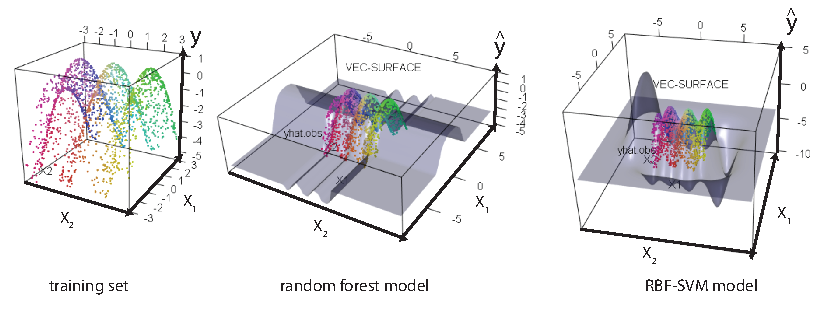
\includegraphics[width=\textwidth,height=\textheight,keepaspectratio]{graphics/svmVSrf.pdf}
\caption{Left plot, a training set has been simulated from $y = sin(x_1 \pi) − \frac 1 2 x_2^2$ where $x_1$ and $x_2$ are drawn from an uniform distribution within $[-3;3]$. Middle and left plot, RF and RBF-SVM have respectively been trained on the data set, providing two completely similar model structures within the proximity of training data. The the shape of the RF and RBF-SVM model structures heavily disagree outside training set area. See the simulation code in \ref{CV5_SVM_RF_same_same}.} 
\label{svmVSrf}
\end{figure}

\section{Random Forest}

\subsection{bagging}
Random forest is a bootstrap aggregated ensemble model meaning it is a collection of independently trained sub models, where each model is trained on a bootstrapped sample of the training set. The prediction error of bagged ensemble models can be lower than the average prediction error of the individual models.

Bootstrapping the training set means to sample a random set of observations. This bootstrap set has the same size as training set and could include every observation of the training set. This would be very unlikely. By default (uniform distribution, sampling with replacement) the chance, that an observation is not included, is approximately 37\%. The chance an observation is sampled at least once is \%63, see Appendix \ref{CV9_RFsampling} for an exact sampling description.

For random forest the same learner, decision tree, is bagged perhaps 500 times. The ensemble prediction is typically the average vote of the ensemble. Besides random forest, bagging is an easy way to combine different model approaches to achieve a perhaps lower prediction than any model approach alone. As bagging independently train each model, the computation can easily be distributed across multiple CPUs or nodes in a server cluster. Appendix \ref{CV8_combineBagging} provides an elaborate parallel implemented example, where logistic regression is combined with random forest to form a new and more accurate ensemble.

When only bagging multiple linear regression models, the acquired ensemble can actually be reduced to one linear regression model where each coefficient is the average of the corresponding coefficients in each sub model. Hereby bagging provides a regularized model similar to increasing the $lambda$-parameter of elastic net and where $alpha=1$. For ensembles of non-linear models, there are no obvious average model. However the bagging still provide regularization, offering a more robust model estimation, than a single learner model alone.

\subsection{Introduction to decision trees}
The random forest algorithm is an improvement of the classification and regression tree algorithm (CART) \cite{breiman1984classification,breiman2001random}. The individual decision trees of random forest are built by applying a collection of steps recursively.

\begin{enumerate}  
\item A collection of observations is called a node and a node has a prediction, that is the average target. A node is terminal, either as there are no valid features left to split by or if a stop criterion has been triggered. Stop criteria are: Exceeding max allowed nodes in tree (infinite by default), reaching minimal allowed node size (5 for regression, 1 for classification), or if all targets are the same.

\item For any intermediary node, a split rule is defined by a break point. For a break point for a given numeric feature, any observation having a feature value below or equal is forwarded to a left daughter node and otherwise to a right daughter node. Every possible split will be tried. For categorical features, any unique separation of categories into two daughter nodes will be tried.

A loss function evaluates and select the best split. By default the loss function is the sum of squared residuals for regression and a variation of gini-index for classification. The regression loss function choose the split, that maximizes the variance across daughter nodes and minimizes intra-daughter node variance. The classification loss function choose the split that produces two nodes most unlike a uniform class distribution. The loss function implementation is discussed in detail in Appendix \ref{CV11_RFginigain}.

\item For each daughter node restart the procedure from step 1.

\end{enumerate}

In Figure \ref{simpleTree} a simple regression tree is built. Left side shows a geometrical representation of the model structure. Right side shows a graph representation of the same model. The nodes are enumerated as these are created. For a CART tree, the training set and root node is not the same, as all observations is used to build the tree. In a random forest ensemble, all trees share the same training set. The training observations passed to each root node of each tree is a bootstrap of the training set. The root node is split into node 2 and node 3. The recursive algorithm proceed with daughter node 2 first (left). If left node is terminal, the algorithm will return to parent node and proceed to right daughter node. If right daughter node is terminal, the algorithm will return to parent-parent node. Therefore the algorithm will visit the nodes in this sequence: root - 2 - 4 - 2 - 5 - 2 - root - 3 - 6 - 3 - 7 - 3 - root.

\begin{figure}[!htbp]
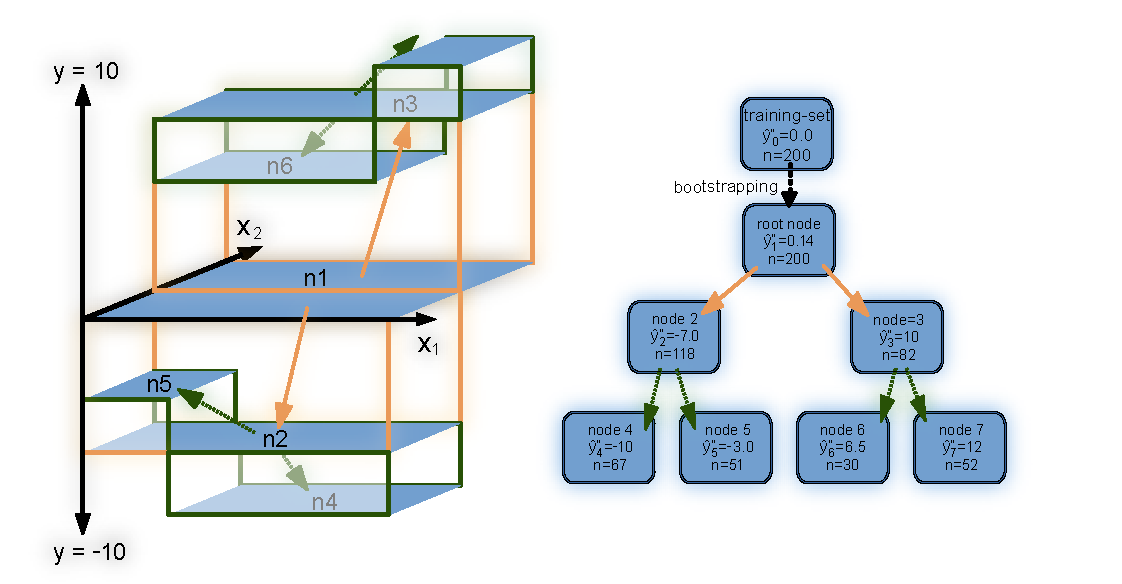
\includegraphics[width=\textwidth,height=\textheight,keepaspectratio]{graphics/randomForest_explained_thesisVersion.pdf}
\caption{Two representations of the same model tree. Left, a geometrical representation of the model surface. Right, a graph representation of the same tree model. Nodes are enumerated as created by the learning algorithm. $\hat{y}^{''}_j$ are the node predictions. $n$ is the node size. $X_1$ and $X_2$ axes are two numerical variables and $y$ axis the prediction axis. This figure is copied and modified from \cite{welling2016forest}.}
\label{simpleTree}
\end{figure}

Although decision trees are a collection simple univariate binary step functions, the stacked trees can ideally estimate almost any structure including interactions. The tree example of Figure \ref{simpleTree}, do in fact contain an interaction where high $X_1$ give a higher terminal prediction, when $X_2$ is also high, and the opposite if $X_2$ is low. In appendix\ref{CV4_assertInteraction} there is a simple simulation verifying that random forest can fit interactions.

Whereas a two-way interaction term in a multiple linear regression is simply defined as  $\hat{y} = \beta_0 + \beta_{12} x_1 x_2 + ...$, the interactions of decision trees are not easy to comprehend when represented as an equation of stacked step functions. It is neither easy to comprehend the interactions by a graph representation, especially when the trees have more than 50 nodes. This has led to that interactions are only vaguely defined and discussed for random forests \cite{boulesteix2014letter}. In Section \ref{defineInteractions}, I argue product interaction terms as known from linear regression, cannot represent any type of interactions in random forest models. Also, I provide my geometrical definition of interactions in random forest models.

Although random forest is a powerful learning algorithm to estimate interactions for a series of data problems, there is a limit for how complex an interaction the random forest learning algorithm can fit. Although a given tree with a very high number of nodes could potentially approximate any model structure, the random forest algorithm cannot necessarily grow that tree, because the loss function consider only the immediate best univariate split. In Section \ref{forestFloorSuppl}, \textit{Supplementary materials for "Forest Floor Visualizations of Random Forest - 1.3 Shallowness of Random forest"} there are provided examples of high-order interactions, that random forest cannot fit. This is the reason why neural networks will supersede random forest when a very complex model structure is needed.

\subsection{Regularization in random forest}
Single fully grown decision trees have a low bias, meaning the learning algorithm is flexible enough to build a model to approximate almost any function, if there is enough training observations and the noise level is low. However as mentioned, decision trees cannot fit high-order interactions, see Section \ref{forestFloorSuppl}. If the function to approximate is not a step function itself, but some rounded structure, it will take high number terminal nodes to approximate. Similarly it takes a high number of square pixels to draw a seemingly round circle on a screen. To obtain the lowest bias, the decision tree must be fully grown. Unfortunately, when every terminal node prediction is made up by only one observation, the model will be noise labile. For the rare occasion of noise free data sets, a single fully grown decision tree can work well. In Figure \ref{decisionTreeFit}, to the left a noise free data set simulated by the function $y=(X_1^2 + X_2^3)^2 - (X_1^2 + X_2^3)$, where $X_1$ and $X_2$ are drawn from uniform distributions. To the right, a decision tree with one observation per terminal node. Overall the decision tree approximate the underlying function well, the cross-validated explained variance is 96\%.

\begin{figure}[!htbp]
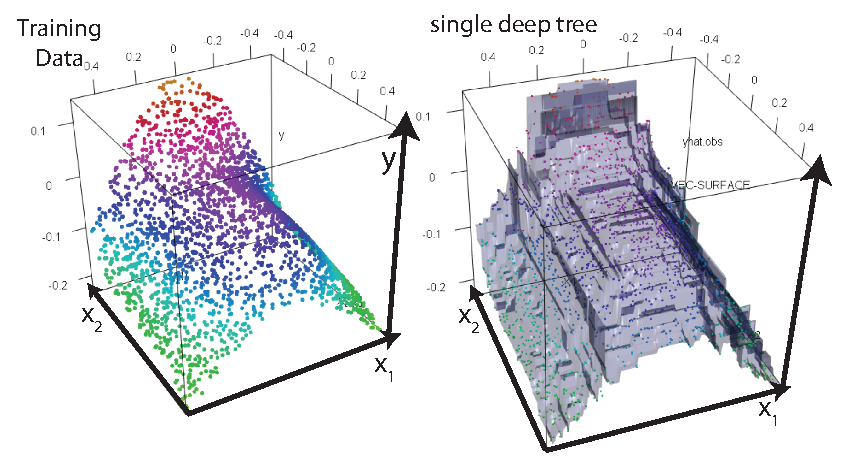
\includegraphics[width=\textwidth,height=\textheight,keepaspectratio]{graphics/decisionTreeFit.pdf}
\caption{Single regression tree fit to 2500 data points without noise. $y=(X_1^2 + X_2^3)^2 - (X_1^2 + X_2^3)$, where $X_1$ and $X_2$ are drawn from uniform distributions.}
\label{decisionTreeFit}
\end{figure}

If the same data set is added a normal distributed noise on the target values, the model variance in its predictions will rise up. In Figure \ref{allTrees}, the same simulated data set has been added noise to the target, such that 33\% of the variance is non explainable noise. An optimal model would therefore be able to explain approximately 67\%. Model (a) is a single fully grown decision tree. The cross-validated explained variance is however only 30\%. In model (b), the decision tree is regularized by limiting the depth of the decision tree, such that no node will be split if having less than 150 observations. The cross-validated explained variance is 50\%. The model is no longer unstable, however as seen in the Figure \ref{allTrees}, the model is now very crude and square. Thus by a bias-variance trade-off, the model have become stable by constraining the model surface complexity. Ensemble regularization with bagging can lower the decision tree variance without increasing the bias as much.  Model (c) is a default random forest model, minimal nodesize = 5, number of trees is 500. The cross-validated explained variance of the model is 60\%. The default RF model structure surface still contain some random ripples that attributes to the model variance. To regularize the model beyond a default random forest model, there are four approaches: random variable sub space(see next section), bootstrap size, terminal node size and max nodes. As with model (b) the tree depth can be limited by restricting minimal node size or max nodes. In model (d) a trees of the random forest are limited to a minimal nodes size of 50. No node with less than 50 observations will be split. To increase the robustness of RF models directly by limiting the depth of each tree is recommended e.g. in Elements of Statistical Learning \cite{friedman2001elements} and in this simulation yields a cross-validated explained variance of 63.5\%. However I find, when limiting tree depth directly, the tree correlation increases. Visually model (d) seems smoothed compared to (c). However model (d) also seems to retain some bias similar to the structure of model (b). Limiting bootstrap sample size to e.g. 10\% of $N$ training observations instead will also lower the tree depth as fewer splits can be made before each tree is fully grown. The tree correlation will be very low, as each bootstrap are much more different. Model (e) is a random forest where bootstrap sample size has been lowered to 250 instead of 2500, the model structure appear even more rounded and the cross-validation explained variance is 64.5\%, slightly better than standard way to regularize RF. The slightly lower prediction error of model (e) over model (d) comes with a price. In Appendix \ref{CV12_RFsampsize} a simulation show sample size regularization requires more trees to converge to a minimal prediction error, than with node size regularization as recommended by Friedman \textit{et al}. In terms of training speed, fewer observations per tree approximately cancels the more trees required. This finding is interesting as sample size regularization, seem not to be mentioned much in random forest literature.

\begin{figure}[!htbp]
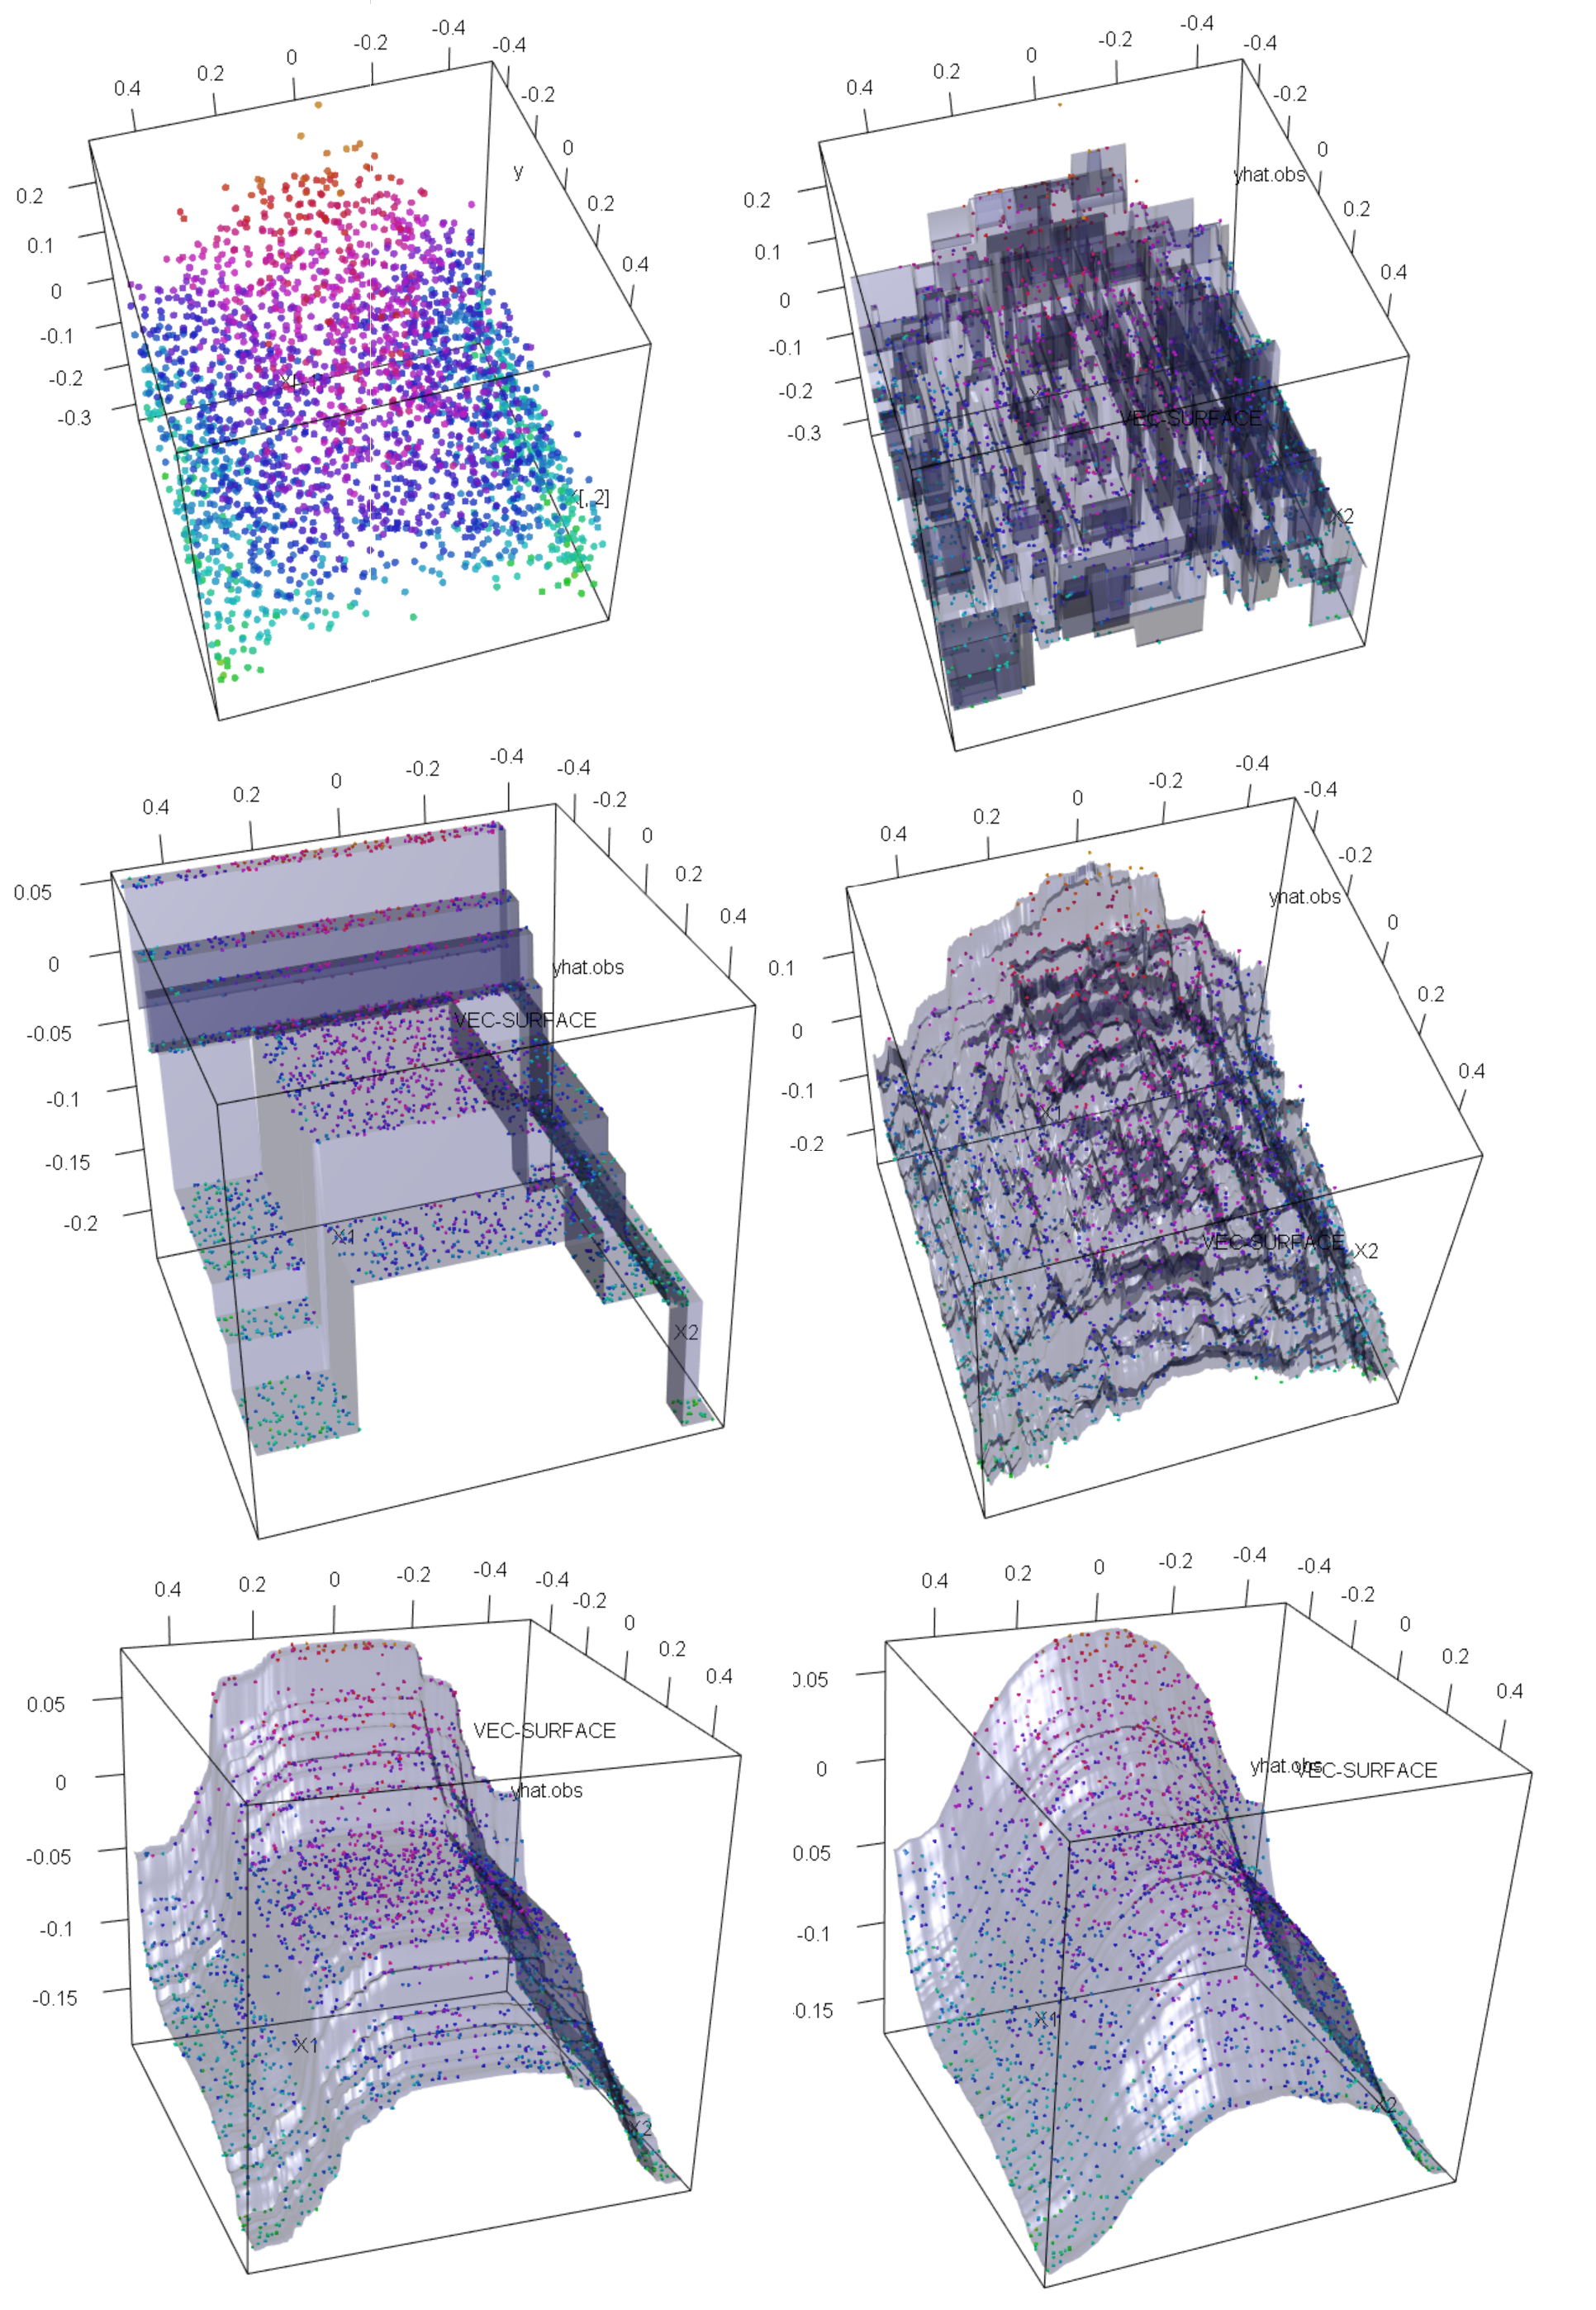
\includegraphics[width=\textwidth,height=\textheight,keepaspectratio]{graphics/allTrees.pdf}
\caption{Single regression tree fit to 2500 data points with a 33\% unexplainable noise/variance component, $y=(X_1^2 + X_2^3)^2 - (X_1^2 + X_2^3)$, where $X_1$ and $X_2$ are drawn from uniform distributions. (a) single tree, min node size is 5 , (b) single tree, min node size is 150, (c) ensemble of 500 trees, min node size is 5, (d) ensemble 1500 trees, min node size is 50, (e) ensemble of 1500 trees, min node size is 5, bootstrap sample size is 250}
\label{allTrees}
\end{figure}

\subsection{Random subspace regularization}
Node size and sample size regularization as seen in Figure \ref{allTrees} tend to smooth the model structure. A third type of regularization is central for the random forest algorithm, called random variable subspace regularization. At any split only a random sample of features (aka. variables) are available to split by. This hyper parameter is called \textit{mtry}, relating to the feature training matrix of $n$ rows and $m$ columns. If \textit{mtry} is 3, only three random columns can be accessed by the algorithm for any split. Setting \textit{mtry} = 1, will force the algorithm to use all features evenly. Setting \textit{mtry} equal to the total number of features will allow the algorithm to greedily split by one dominant feature first and then only deeper down the tree make minor corrections by other features. Therefore random variable subspace regularization have a similar effect as $L2$-regularization of elastic net. A low \textit{mtry} tend to distribute the dependence on features. Moreover, a low \textit{mtry} decrease the tree correlation as different features will be used to make the first split. However low \textit{mtry} tend to increase bias, especially interactions are fitted less well. In Appendix \ref{article:solubility} model structures are visualized for different values of \textit{mtry}.

\subsection{Final choice of regularization}
The standard approach is to find the set of hyper parameters that give the lowest cross-validated prediction error. However, already by visually inspecting the model surface, the user should consider if the model surface is plausible.  Would it be realistic to reproduce e.g. the complex surface of model (a) and (c), if a new data set was sampled. If the user in fact expect the underlying function to be complex and the unexplainable noise component to be low, then the user should lean towards a model with less regularization and accept model (c). If the user expect the noise component to be substantial, then the user should lean towards more regularization, as a complex model structure would be unrealistic to estimate. Also as discussed in Section \ref{unbiased_estimation}, model selection may be misleading. The model selected by the validation set, could be mostly selected due to luck and not skill. Luck happens to regress towards the average, it cannot be reproduced \cite{kahneman2011thinking}. Therefore, there is no standard cross-validation procedure that can calibrate any model. The user must inevitably include her own expectation to the underlying function that generates the data.

Moreover in terms of communication, the user can regularize the model beyond what seems optimal to lower the prediction error, as the model structure especially when high-dimensional may be easier to explore and communicate. An over regularized random forest model structure may be easier to visualize and yet far more accurate, than a linear regression model.